\documentclass{article}

\usepackage[utf8]{inputenc}
\usepackage{polski}
\usepackage{titlesec}
\usepackage{graphicx}
\usepackage[hidelinks]{hyperref}

\graphicspath{{images/}}

\title{Generator ruchu Google Analytics \\ Iteracja II architektura systemu}
\author{Bartłomiej Dalak \and Bartłomiej Karwowski \and Bartosz Gromek \and Tomasz Kanas}

\begin{document}
\maketitle

\section{Wstęp}

Dokument architektury systemu ma na celu przedstawienie wizji architektury. Opisana architektura może ulec zmianom w fazie implementacji.

\section{Aplikacja}

Aplikacją będzie system kolejkowania wysyłania wejść na podaną stronę użytkownika do Google Analytics.

\section{Opis elementów architektury}

\subsection{UI}
Użytkownik po wejściu na stronę zobaczy po lewej stronie listę wszystkich zadań dodanych do systemu, podzieloną na 2 kolumny. W pierwszej będzie id zadania, w drugiej stan w jakim się znajduje. W dalszej częsci dokumentu będzie opisany każdy stan. Pod listą znajduje się przycisk \textbf{Add new} pozwalający dodać nowe zadanie ze statusem \textbf{NEW}. Automatycznie po prawej stronie pokaże się formularz gotowy do uzupełnienia. Po uzupełnieniu go, będzie mógł go zapisać naciskając przycisk \textbf{Save}. Zmieni się wtedy stan na \textbf{READY}. Dodatkowo użytkownik naciskając na wiersz listy, będzie mógł zobaczyć szczegóły wybranego zadania. Jeśli będzie to zadanie w stanie \textbf{READY}, będzie można edytować dane. Dodatkowo pojawi się przycisk \textbf{Delete} obok przycisku \textbf{Save} pozwalający usunąć zadanie do wykonania. Jeśli będzie to zadanie w stanie \textbf{IN PROGRESS}, to pojawi się przycisk \textbf{Cancel} pozwalający przerwać wykonywanie zadania. 
\subsubsection{Przykładowy wygląd}
\begin{center}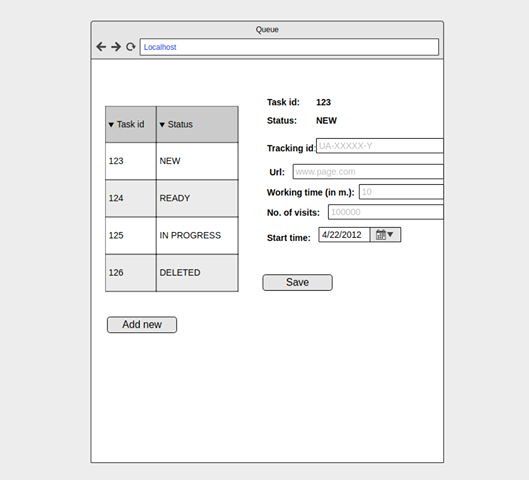
\includegraphics[scale=0.75]{ui}\end{center}

\subsubsection{Stany zadań}

\begin{itemize}
\item \textbf{NEW}: zadanie dodane do bazy
\item \textbf{READY}: zadanie zapisane, czekające na wykonanie
\item \textbf{IN PROGRESS}: zadanie w trakcie wykonywania
\item \textbf{CANCELED}: zadanie zatrzymane
\item \textbf{DELETED}: zadanie usunięte, zanim zaczęło się wykonywać
\item \textbf{DONE}: zadanie zostało wykonane
\item \textbf{ERROR}: wystąpiły problemy w trakcie wysyłania
\end{itemize}

\subsubsection{Przejścia stanów}
\begin{center}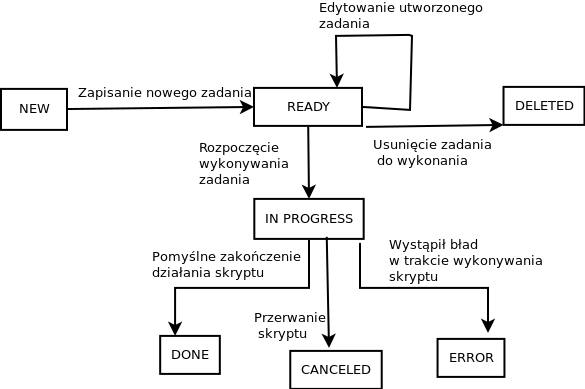
\includegraphics[scale=0.5]{states_diagram}\end{center}

\subsection{Baza danych}

Jako systemem do zarządzania bazą użyjemy SQLite. Baza będzie zawierała dwie tabele:
\begin{itemize}
\item \textbf{state}, która będzię trzymała stany w jakich może znajdować się zadanie. Będzie sie składała z 2 kolumn:
\begin{itemize}
\item \textbf{id: INT}: id statusu
\item \textbf{name: TEXT}: nazwa statusu
\end{itemize}
\item \textbf{tasks}, która będzie trzymała dodane zadania. Kolumny z jakich będzie sie składać:
\begin{itemize}
\item \textbf{task\_id: INT, PK}: id zadania
\item \textbf{tracking\_id: TEXT}: tracking id użytkownika
\item \textbf{url: TEXT}: url strony na jaką chcemy dodawać użytkowników
\item \textbf{time: INT}: czas przez jaki ma działać skrypt
\item \textbf{visits: INT}: liczba użytkowników do wygenerowania
\item \textbf{start\_time: DATE}: data kiedy ma się wykonać skrypt
\item \textbf{state: FK do state.id}: klucz obcy do tabeli stanów oznaczający stan w jakim aktualnie znajduje się zadanie
\end{itemize}
\end{itemize} 

\subsection{Backend aplikacji}
Słuzy do komunkacji między \textbf{UI}, a \textbf{bazą}. Użyjemy do tego frameworka \textbf{Flask}. Będziemy używać widoków:
\begin{itemize}
\item widok pod adresem ``/tasks'' z metodą \textbf{GET} wyświetlający listę wszystkich zadań
\item widok pod adresem ``/tasks'' z metodą \textbf{POST}, który będzie dodawał nowe zadanie do bazy, odświeżał listę wyświetlonych zadań i wyświetlał formularz
\item widok pod adresem ``/tasks/save'' z metodą \textbf{POST}, który będzie aktualizował wybrane zadanie i dodatkowo walidował czy został podany poprawny \textbf{tracking\_id}
\end{itemize}

\subsection{System kolejkowania}
\subsubsection{Język}
Python 3.6. 
\subsubsection{Użyte biblioteki}
\begin{itemize}
	\item \textbf{multiprocessing}: Tworzenie nowych procesów wysyłających dane do GA, oraz zarządzanie nimi.
\end{itemize}
\subsubsection{Opis działania}
Skrypt, który co 1 minutę będzie wysyłał zapytania do bazy pobierając dane. Skrypt będzie sprawdzał, czy należy uruchomić kolejny proces (czy rozpoczęło się właśnie nowe zadanie), czy jakiś działający proces należy przerwać (użytkownik go anulował), oraz monitorował działanie wszystkich procesów i aktualizował w bazie danych ich stan w przypadku jego zmiany --- zakończenia działania (sukces lub błąd).

\subsection{Skrypt do wysyłania zapytań do GA}

\subsubsection{Język}

Wykorzystany zostanie Python w wersji 3.6.

\subsubsection{Użyte biblioteki}

\begin{itemize}
\item \textbf{requests}: wysyłanie zapytań do GA i Measurement Protocol Validation Server
\item \textbf{csv}: do obsługi pliku `browser.csv', w którym mamy rozkład przeglądarek na terenie Polski.
\end{itemize}

\subsubsection{send\_requests\_api}
API służące do komunkacji z GA, generuje potrzebne dane oraz je wysyła.
Dostępne metody:
\begin{itemize}
\item \textbf{send (tracking\_id, url, visits\_no, time)}: Przekazuje dane do niżej opisanej funkcji \textbf{generate\_data}. Po odebraniu wygenerowanych danych, próbuje przesłać je bezpośrednio do GA\@. Przykładowe wysłanie danych: \textbf{requests.post (``https://www.google-analytics.com/\\collect'', data={``v'':  1, ``t'': ``pageview'', ``tid'': tracking\_id, ``cid'': 1, ``dp'': url})}. W ten sposób będziemy wysyłać w pętli kolejne wejścia z wygenerowanych danych. Zwraca kod \textbf{OK}, po wygenerowaniu wszystkich danych.

\item \textbf{generate\_data (visits\_no)}: metoda wołana przez \textbf{send ()}, generujące odpowiednie dane do wysłania. Po odebraniu informacji przekazanych przez użytkownika, do odpowiedniej ilości zapytań przypisuje dane przygotowane z wiarygodnym rozkładem. Informacje do tego potrzebne zostaną zczytane z pliku `browser.csv', który zostanie pobrany ze strony \href{http://gs.statcounter.com/browser-version-market-share/all/poland#monthly-201703-201803-bar}{GlobalStats StatCounter (dane\ dot.\ oprogramowania\ użytkowników\ witryny)}. Informacje te zostaną przypisane na zmienną \textbf{distribution\_informations} będącą typu DataFrame. Zostanie to wykonane tylko raz.
\end{itemize}

\subsubsection{Wykres użytkowania przeglądarek na terenie Polski}
\begin{center}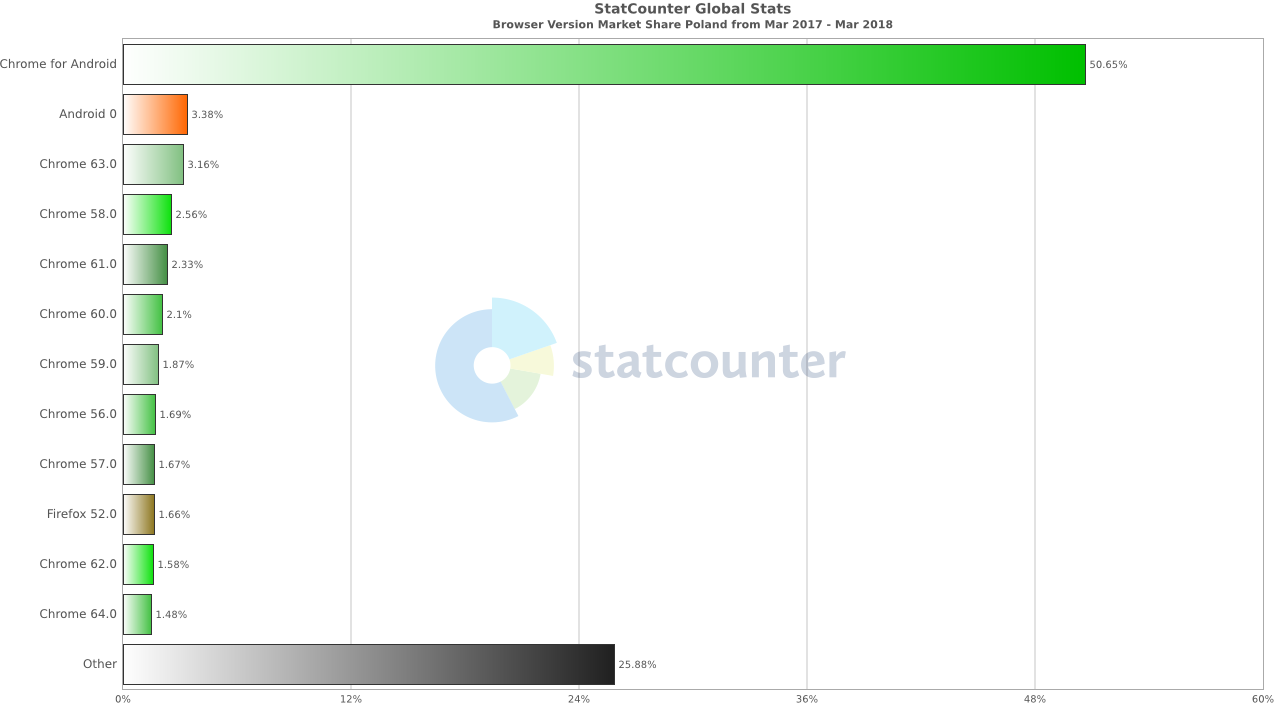
\includegraphics[scale=0.25]{chart}\end{center}

\subsubsection{Schemat działania}

\begin{itemize}
\item \textbf{przekazanie danych}:
Użytkownika wywołuję funkcję \textbf{send (tracking\_id, url, visits\_no, time)} udostępnioną przez \textbf{send\_requests\_api}. W rezultacie otrzymuje komunikat tego czy udało się pomyślnie wysłać żądanie.

\begin{center}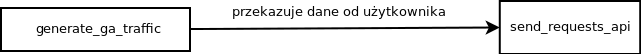
\includegraphics[scale=0.5]{put_data}\end{center}

\item \textbf{wygenerowanie danych}
Po otrzymaniu danych od użytkownika zostaje wywołana funkcja \textbf{generate\_data}, która generuje i zwraca dane. 

\begin{center}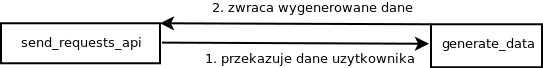
\includegraphics[scale=0.5]{generate_data}\end{center}

\item \textbf{wysyłanie danych i zwrócenie komunikatu}
Po otrzymaniu wygenerowanych danych zostają one wysyłane do Google Analytics, a następnie zostaje zwrócony komunikat powodzenia.

\begin{center}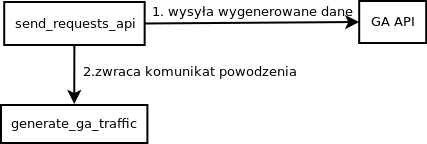
\includegraphics[scale=0.5]{send_data}\end{center}
\end{itemize}

\section{Komunikacja między elementami}
\subsection{UI, backend aplikacji i baza danych}
\begin{center}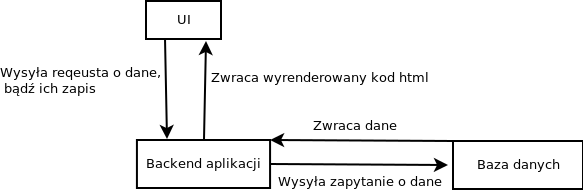
\includegraphics[scale=0.5]{ui_b}\end{center}

\subsection{System kolejkowania, baza danych i skrypt}
\begin{center}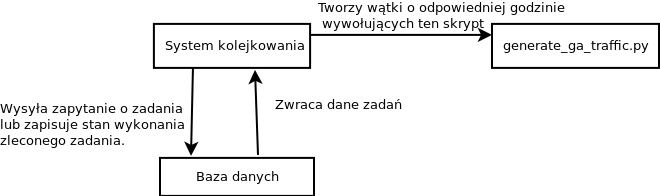
\includegraphics[scale=0.5]{system}\end{center}


\end{document}
